\documentclass[a4paper,
12pt,
BCOR12mm,
]{scrartcl}
%scrreport
\usepackage[ngerman]{babel}
\usepackage[utf8]{inputenc}
\usepackage[T1]{fontenc}
\usepackage{url}
\usepackage[pdftex]{graphicx}
\usepackage{listingsutf8}
\usepackage{grffile}
\usepackage{epstopdf}
\usepackage{subfigure}
\usepackage[a4paper,left=23mm,right=23mm, top=33mm, bottom=66mm]{geometry}
% lstlisting settings
\lstset{
showspaces=false,
breaklines=true,
breakindent=0pt,
frame=single,
language=C,
extendedchars=true,
inputencoding=utf8/latin1,
identifierstyle=\ttfamily,
basicstyle=\tiny,
numbers=left,
numberstyle=\tiny,
}

\title{APUVS, Blatt 4}
\author{Jan Fajerski and Kai Warncke and Magnus Müller}

\begin{document}
% NOTE: compile with pdflatex --shell-escape main.tex

\maketitle 

\section*{Aufgabe 4.1}

% some graphs
\begin{figure}[!h]
	\begin{center}
		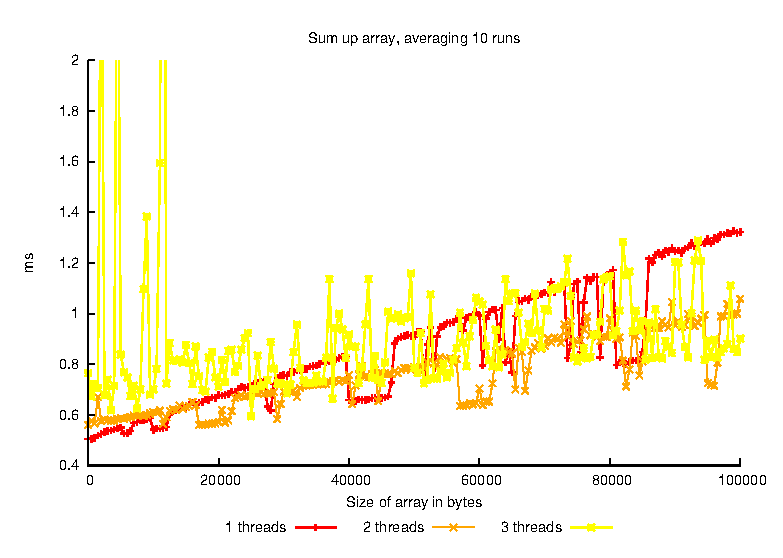
\includegraphics[width=\textwidth]{../a_4_1/graphs/summation_1st}
	\end{center}
	\caption{Summation mit 1-3 Threads}
	\label{fig:summation_1_3}
\end{figure}
\begin{figure}[!h]
	\begin{center}
		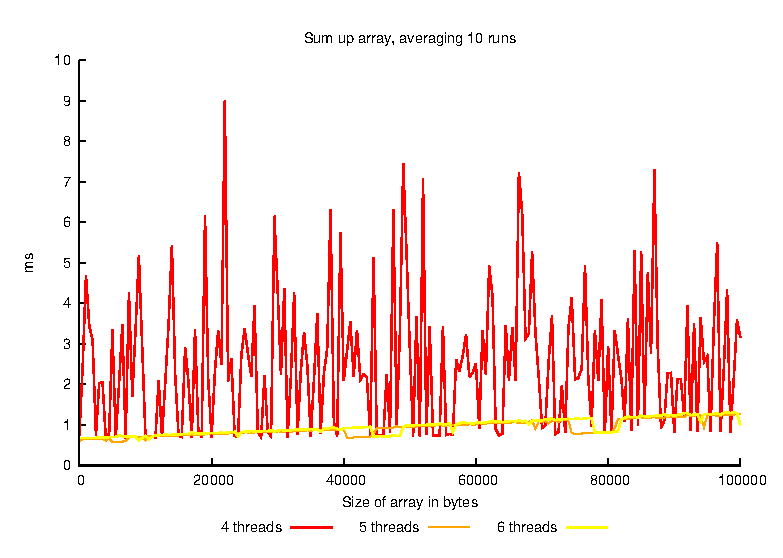
\includegraphics[width=\textwidth]{../a_4_1/graphs/summation_2nd}
	\end{center}
	\caption{Summation mit 4-6 Threads}
	\label{fig:summation_4_6}
\end{figure}
\begin{figure}[!h]
	\begin{center}
		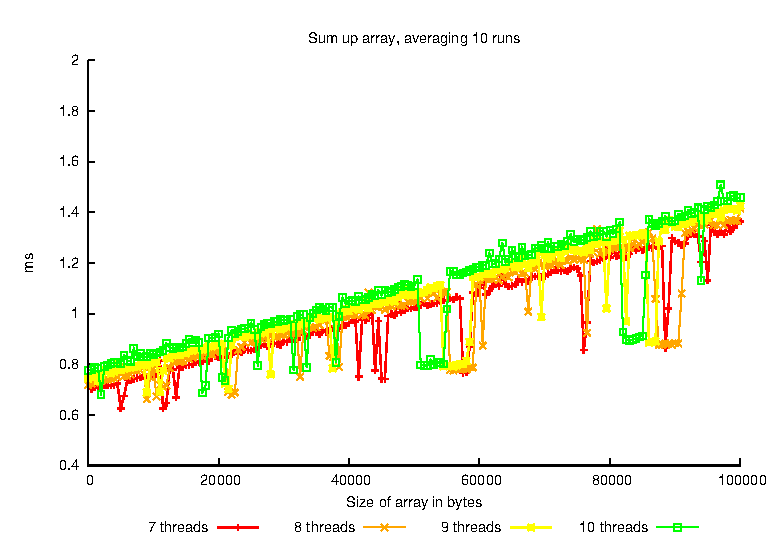
\includegraphics[width=\textwidth]{../a_4_1/graphs/summation_3rd}
	\end{center}
	\caption{Summation mit 7-10 Threads}
	\label{fig:summation_7_10}
\end{figure}

\begin{figure}[!h]
	\begin{center}
		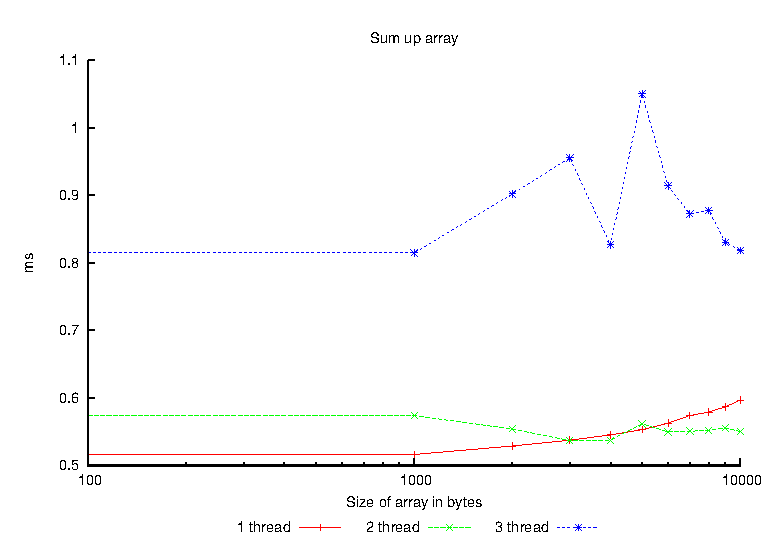
\includegraphics[width=\textwidth]{../a_4_1/graphs/ascending_1st}
	\end{center}
	\caption{Summation aufsteigender Zahlen mit 1-3 Threads}
	\label{fig:summation_1_3}
\end{figure}
\begin{figure}[!h]
	\begin{center}
		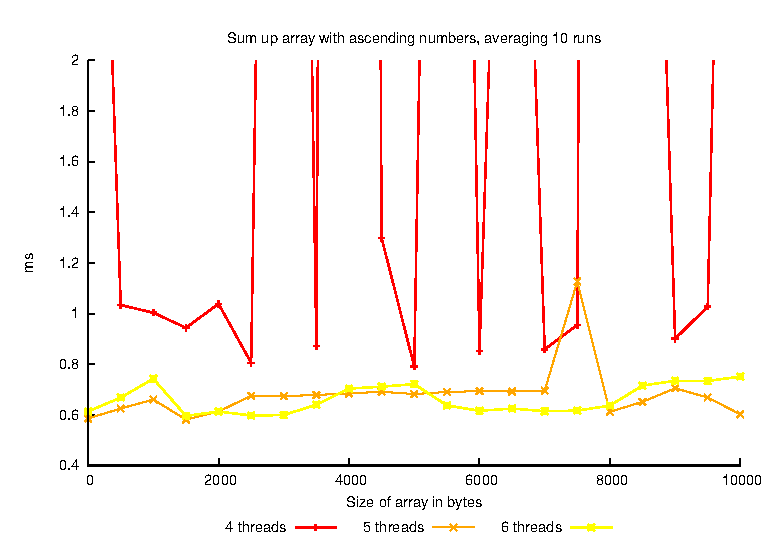
\includegraphics[width=\textwidth]{../a_4_1/graphs/ascending_2nd}
	\end{center}
	\caption{Summation aufsteigender Zahlen mit 4-6 Threads}
	\label{fig:summation_4_6}
\end{figure}
\begin{figure}[!h]
	\begin{center}
		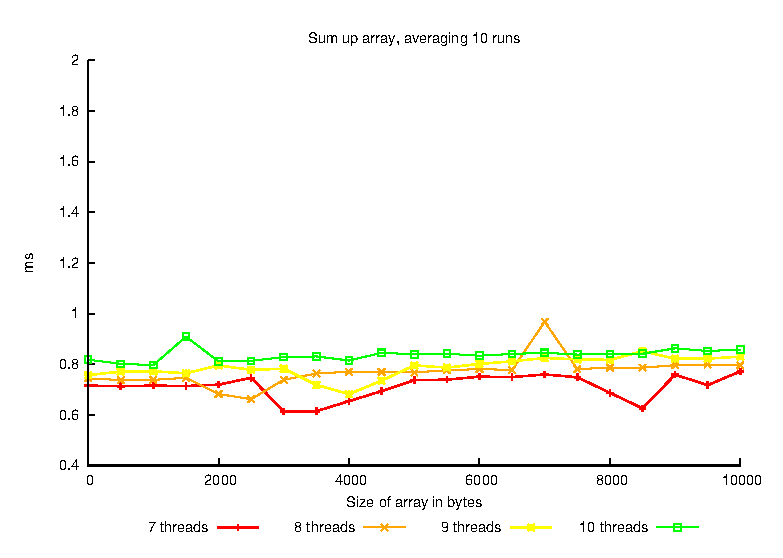
\includegraphics[width=\textwidth]{../a_4_1/graphs/ascending_3rd}
	\end{center}
	\caption{Summation aufsteigender Zahlen mit 7-10 Threads}
	\label{fig:summation_7_10}
\end{figure}
\end{document}
